\section{Approach}

% Algorithmic Design

\begin{frame}{Variables} % ____________________________________________________

Description of the main variables

  \begin{table}[h]
    \begin{center}
      \begin{tabular}{c|l}
      \cellcolor{white} Variable Name & Description \\ % adding \cellcolor{} here fixes the vertical line between the columns for some reason
      \rowcolor{LightGray}
      $D$ & Depth image from RGB-D sensor \\
      $P$ & Pose of the sensor \\
      \rowcolor{LightGray}
      $D_n$ & Parts of $D$ that are \emph{novel} \\
      $S$ & Novel surface generated from $D_n$ \\
      \rowcolor{LightGray}
      $M$ & Global mesh \\
      \end{tabular}
    \end{center}
  \end{table}

\end{frame}

\note[itemize]{
\item Before we begin, let us get familiar with common variable names.
}


\begin{frame}{MABDI Algorithm} % _______________________________________________
  \vspace{-0.15in}
  \begin{center}
  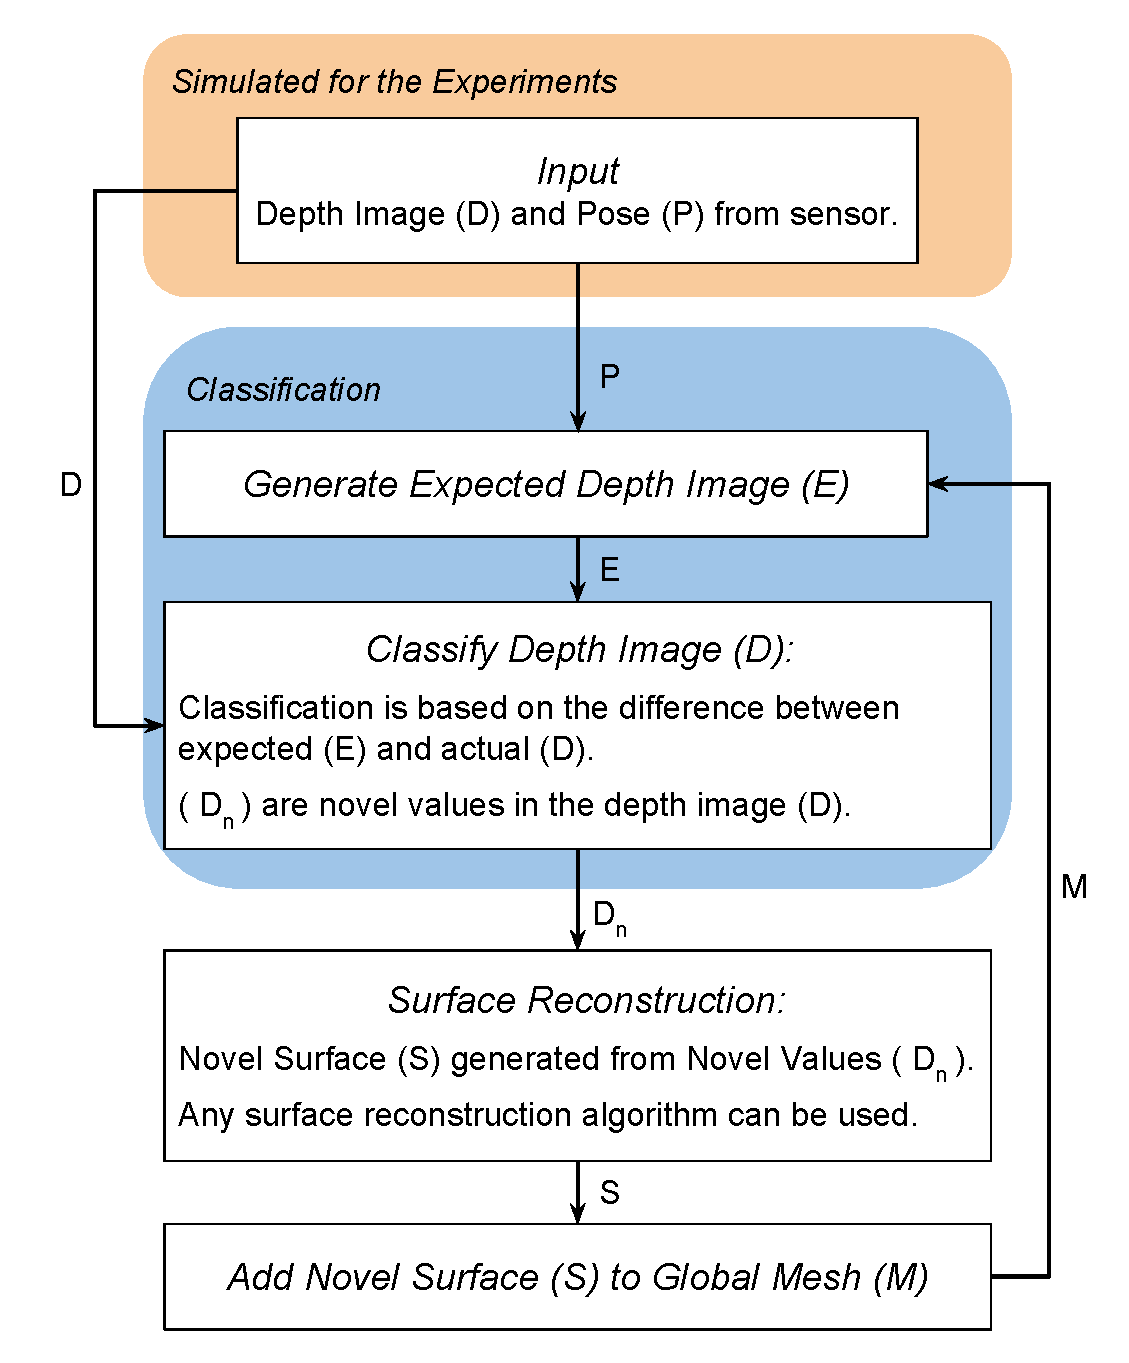
\includegraphics[height=0.95\textheight]{../figures/approach_mabdi_algorithm.pdf}
  \end{center}
\end{frame}

\note[itemize]{
\item[] Input
\item Has been simulated for this work
\item Cover in detail in next section
\item[] Generate Expected Depth Image
\item What we expect to see from our sensor
\item[] Classify Depth Image
\item Determine which points from D are novel
\item[] Surface Reconstruction
\item Create a mesh structure from the novel points
\item Cover in detail next
}

\subsection{Implementation}

% Surface Reconstruction

\begin{frame}{Topology Defined on Depth Image} % _______________________________
\begin{center}
  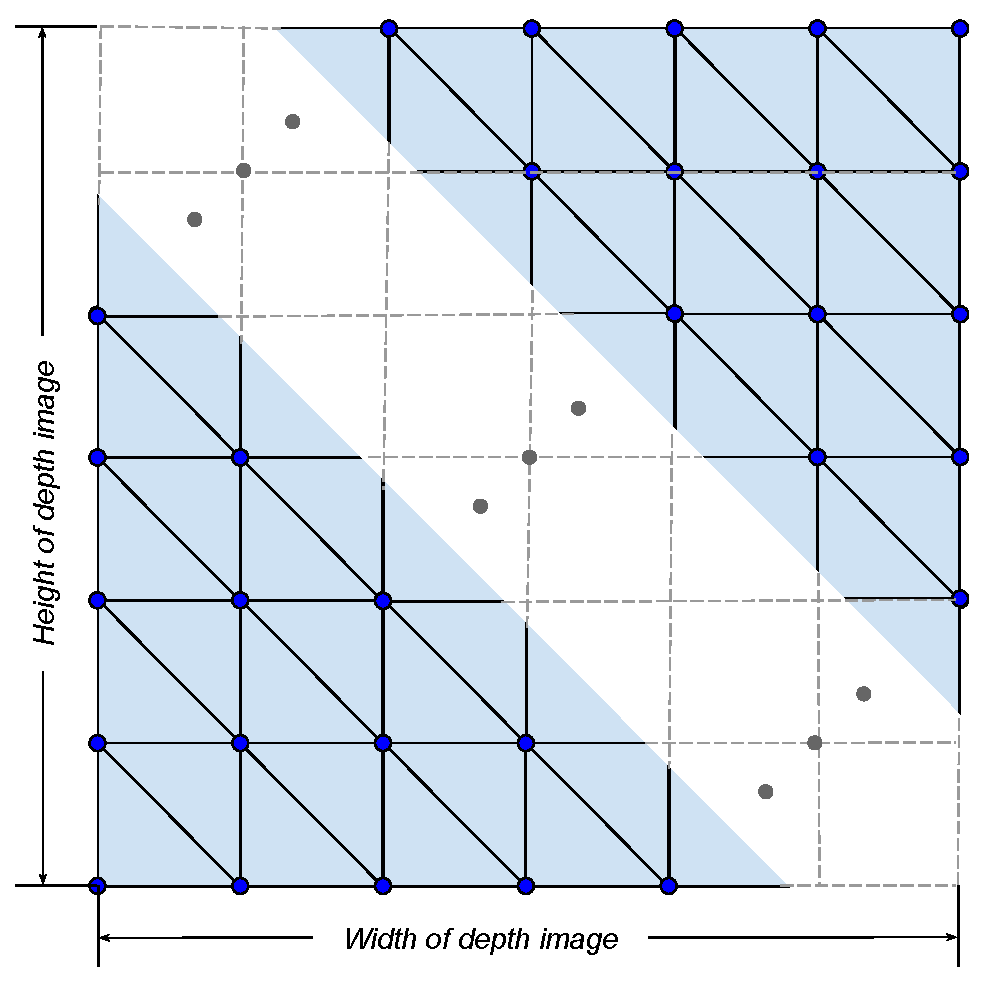
\includegraphics[height=0.90\textheight]{../figures/approach_sr_topology.pdf}
  \end{center}
\end{frame}

\note[itemize]{
\item Mesh consists of vertices and elements
\item - Vertices are points
\item - Elements define connections between vertices
\item Depth image
\item - Not a set of unorganized points
\item - Has structural information
\item - This allows us to define a topology in 2D that is preserved when projected to 3D
}

\begin{frame}{Removing elements} % _____________________________________________
  Elements are removed from the $S$ if they touch pixels from the sets:
  \begin{itemize}
    \item $D_{known}$
    \item $D_{boundary}$
    \item $D_{invalid}$
  \end{itemize}
  % TODO: Venn diagram
\end{frame}

\begin{frame}{Removing elements - $D_{known}$} % _______________________________
  \begin{gather*}
    D_n = \lvert D - E \rvert > threshold \\
    D_{known} = D \setminus D_n
  \end{gather*}
\end{frame}

% Software Design

\begin{frame}{Removing elements - $D_{boundary}$} % ____________________________
  \begin{gather*}
    K = \begin{bmatrix} 2 & -1 \\ -1 & 0 \end{bmatrix} \\
    D_{boundary} = (D \ast K) > threshold
  \end{gather*}
\end{frame}

\note[itemize]{
\item
}

\begin{frame}{Removing elements} % _____________________________________________
  \begin{center}
  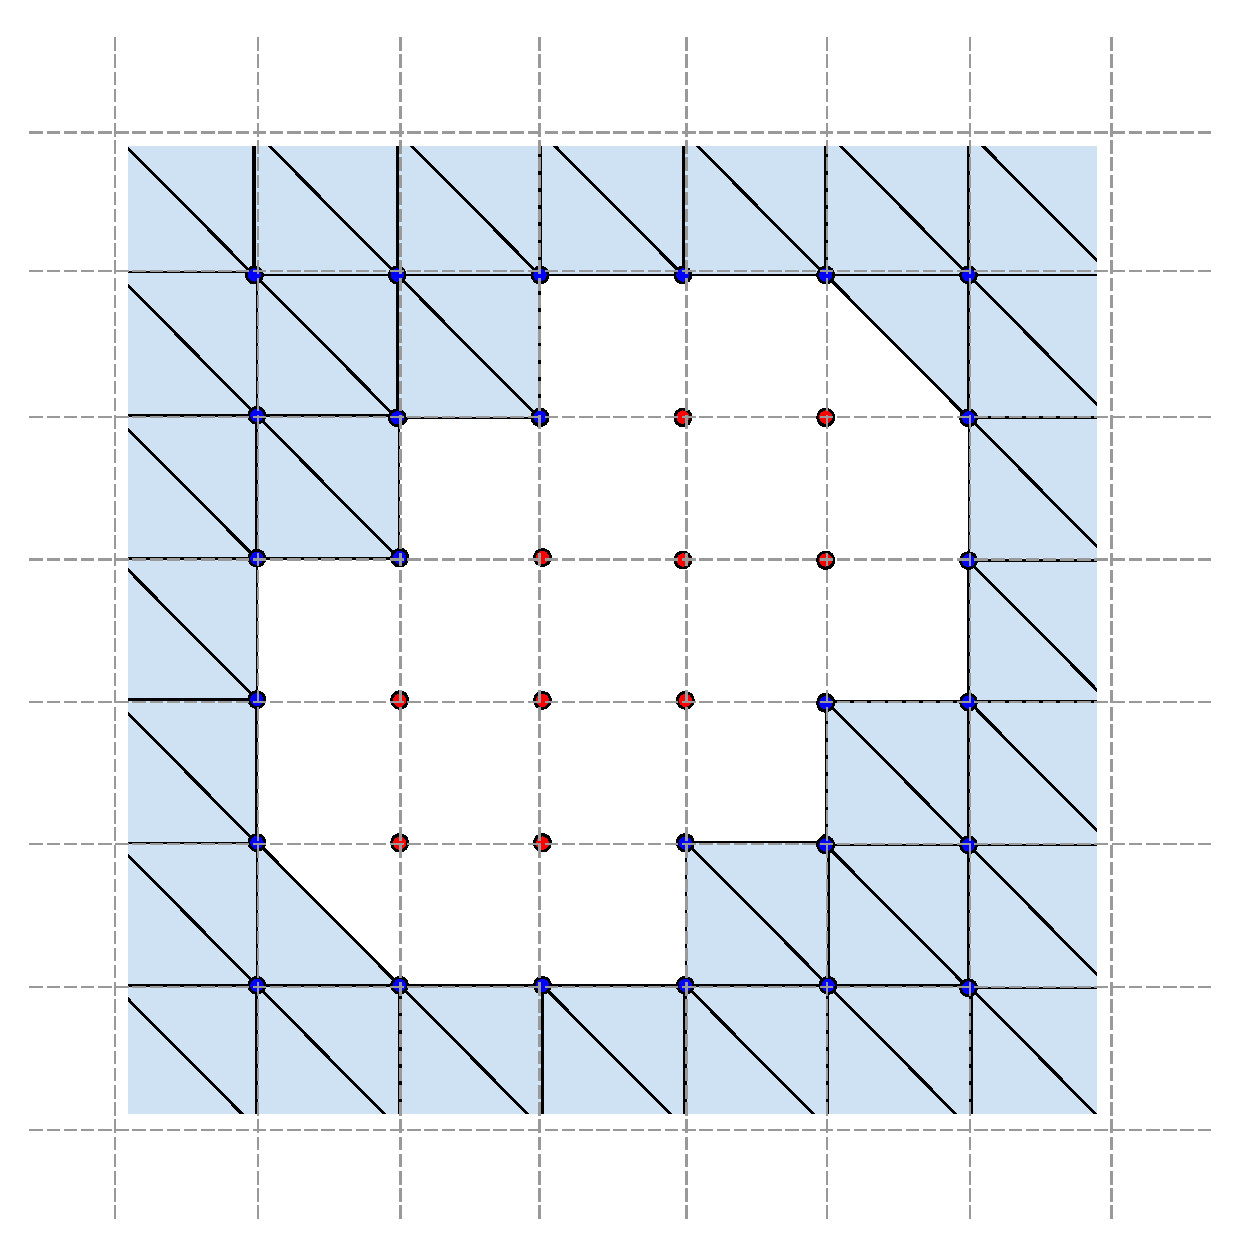
\includegraphics[height=0.90\textheight]{../figures/approach_sr_element_removal.pdf}
  \end{center}
\end{frame}

\note[itemize]{
\item
}

\subsection{Software Design}

\begin{frame}{Diagram} % _______________________________________________________
  \begin{center}
  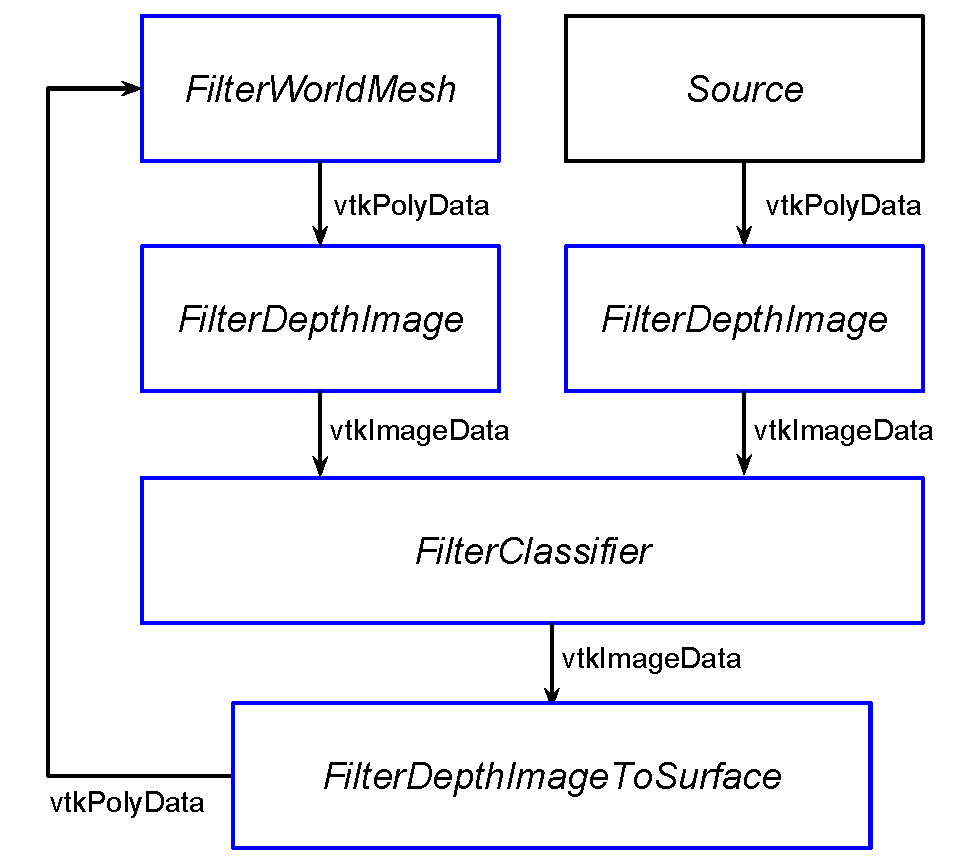
\includegraphics[height=0.90\textheight]{../figures/approach_software_diagram.pdf}
  \end{center}
\end{frame}

\note[itemize]{
  \item  \textit{Source} - Classes with the prefix Source define the
  environment that is used for the simulation and provide a mesh in the form
  of a vtkPolyData.
  \item \textit{FilterDepthImage} - Render the incoming vtkPolyData in a
  window and output the depth buffer from the window as a vtkImageData. The
  output additionally has pose information of the sensor.
  \item \textit{FilterClassifier} - Implements the true innovation of MABDI,
  i.e., takes the difference between the two incoming depth images
  (vtkImageData) and outputs a new depth image where the data that is not
  novel is marked to be thrown away.
  \item \textit{FilterDepthImageToSurface} - Performs surface reconstruction
  on the novel points. The surface is output as a vtkPolyData.
  \item \textit{FilterWorldMesh} - Here we simply append the incoming novel
  surface to a growing global mesh that is also output as a vtkPolyData.
}
